% Block diagram of the uncertainty-aware ensemble, same styles as
% fig_architecture.tex so the two figures read as one family.
%   tectonic -X compile fig_architecture_uncertainty.tex
\documentclass[border=4pt]{standalone}
\usepackage{tikz}
\usepackage{xcolor}
\usepackage{amsmath}
\usetikzlibrary{arrows.meta,positioning,fit,backgrounds,calc}

\definecolor{segfill}{HTML}{DCE9F7}
\definecolor{segline}{HTML}{2A78D6}
\definecolor{confill}{HTML}{FDEBD3}
\definecolor{conline}{HTML}{D9822B}
\definecolor{reffill}{HTML}{DDF2E6}
\definecolor{refline}{HTML}{1B9E6A}
\definecolor{iofill}{HTML}{ECECE8}
\tikzset{
  blk/.style={draw, rounded corners=2pt, align=center, inner sep=3.2pt,
              font=\scriptsize, minimum height=7.5mm, line width=0.5pt},
  seg/.style={blk, fill=segfill, draw=segline},
  con/.style={blk, fill=confill, draw=conline},
  ref/.style={blk, fill=reffill, draw=refline},
  io/.style={blk, fill=iofill, draw=black!55},
  op/.style={draw, circle, inner sep=0.8pt, font=\scriptsize, line width=0.5pt,
             fill=segfill, draw=segline},
  fl/.style={-{Latex[length=1.6mm,width=1.4mm]}, line width=0.5pt, draw=black!70},
  note/.style={font=\tiny, text=black!60, align=center},
}

\begin{document}
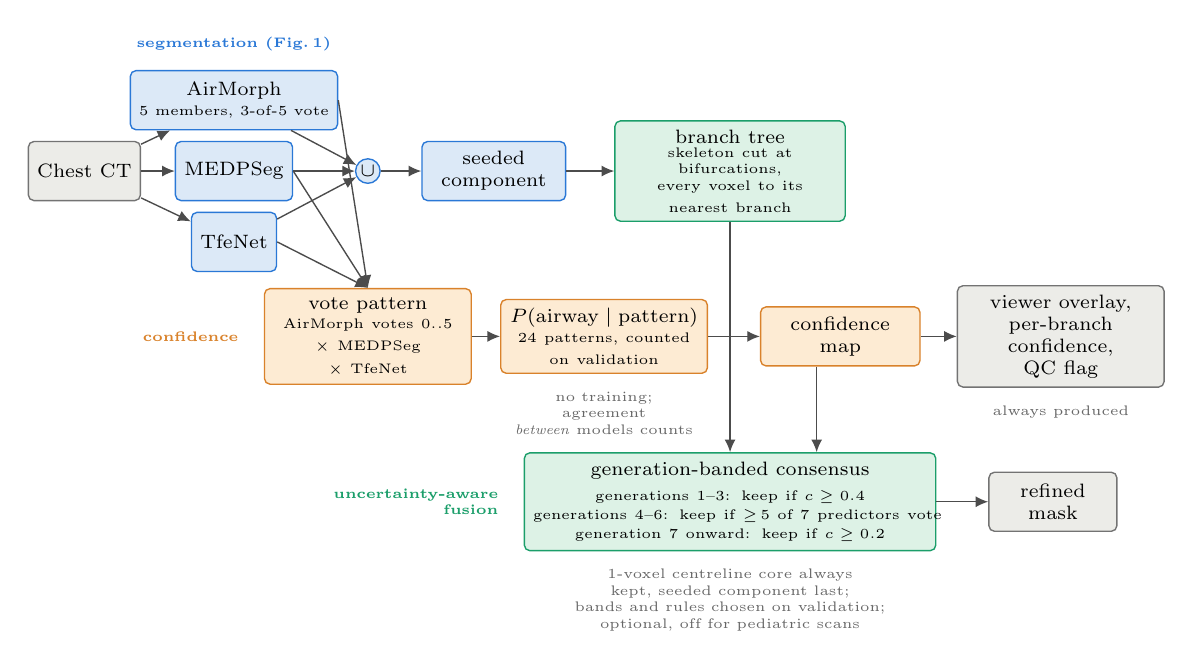
\begin{tikzpicture}

% ---- row 1: the segmentation front end of Fig. 1, then the branch tree
\node[io] (ct) {Chest CT};
\node[seg] (mp) at ($(ct)+(19mm,0)$) {MEDPSeg};
\node[seg] (am) at ($(mp)+(0,9mm)$) {AirMorph\\[-1pt]\tiny 5 members, 3-of-5 vote};
\node[seg] (tf) at ($(mp)+(0,-9mm)$) {TfeNet};
\node[op]  (or) at ($(mp)+(17mm,0)$) {$\cup$};
\node[seg, text width=16mm] (lcc) at ($(or)+(16mm,0)$) {seeded\\component};
\node[ref, text width=27mm] (tree) at ($(lcc)+(30mm,0)$)
  {branch tree\\[-1pt]\tiny skeleton cut at bifurcations,\\[-2pt]\tiny every voxel to its nearest branch};
\draw[fl] (ct) -- (am); \draw[fl] (ct) -- (mp); \draw[fl] (ct) -- (tf);
\draw[fl] (am) -- (or); \draw[fl] (mp) -- (or); \draw[fl] (tf) -- (or);
\draw[fl] (or) -- (lcc); \draw[fl] (lcc) -- (tree);
\node[note, above=1.2mm of am, text=segline] {\textbf{segmentation (Fig.\,1)}};

% ---- row 2: vote pattern -> calibrated probability -> confidence map
\node[con, text width=24mm] (pat) at ($(or)+(0,-21mm)$)
  {vote pattern\\[-1pt]\tiny AirMorph votes $0..5$ $\times$ MEDPSeg $\times$ TfeNet};
\node[con, text width=24mm] (tab) at ($(pat)+(30mm,0)$)
  {$P(\text{airway}\mid\text{pattern})$\\[-1pt]\tiny 24 patterns, counted on validation};
\node[con, text width=18mm] (map) at ($(tab)+(30mm,0)$) {confidence\\map};
\node[io, text width=24mm] (view) at ($(map)+(28mm,0)$)
  {viewer overlay,\\per-branch confidence,\\QC flag};
\draw[fl] (am.east) -- (pat.north); \draw[fl] (mp.east) -- (pat.north); \draw[fl] (tf.east) -- (pat.north);
\draw[fl] (pat) -- (tab); \draw[fl] (tab) -- (map); \draw[fl] (map) -- (view);
\node[note, below=1.0mm of tab, text width=23mm]
  {no training; agreement\\\emph{between} models counts};
\node[note, below=1.0mm of view, text width=26mm]
  {always produced};
\node[note, left=2mm of pat, text width=14mm, align=right, text=conline] {\textbf{confidence}};

% ---- row 3: the refinement, one rule per generation band of the branch tree
\node[ref, text width=50mm] (rc) at ($(tree)+(0,-42mm)$)
  {generation-banded consensus\\[1pt]
   {\tiny\mbox{generations 1--3: keep if $c \geq 0.4$}}\\[-1pt]
   {\tiny\mbox{generations 4--6: keep if $\geq$\,5 of 7 predictors vote}}\\[-1pt]
   {\tiny\mbox{generation 7 onward: keep if $c \geq 0.2$}}};
\node[io, text width=14mm] (out) at ($(rc)+(41mm,0)$) {refined\\mask};
\draw[fl] (rc) -- (out);
\node[note, below=1.0mm of rc, text width=48mm]
  {1-voxel centreline core always kept, seeded component last;\\bands and rules chosen on validation;\\optional, off for pediatric scans};
\node[note, left=2mm of rc, text width=22mm, align=right, text=refline]
  {\textbf{uncertainty-aware\\fusion}};

% the tree supplies each voxel's generation from above, through the gap
% between the table and the map; the map supplies c and the vote count
\coordinate (m1) at ($(map.south)+(-3mm,0)$);
\draw[fl] (tree.south) -- (tree.south |- rc.north);
\draw[fl] (m1) -- (m1 |- rc.north);
\end{tikzpicture}
\end{document}
